\newcommand{\norm}[1]{\left\lVert#1\right\rVert}

%%%%%%%%%%%%%%%%%%%%%%%%%%%%%%
%Ich weiß nicht, wie man dafür sorgen kann, dass die Formeln nicht so komisch aussehen.

\section{Machine Learning}
\author{Farhadiba Mohammed, Dennis Kempf, David Steinmann}
Machine Learning ist ein Konzept, bei dem der Computer durch Algorythmen in der Lage ist Probleme selbstständig zu lösen. Dabei erkennt der Computer nach einer gewissen Lernphase Gesetzmässigkeiten, durch die er dann in der Lage ist, neü, ihm unbekannte Datensätze bezüglich eines bestimmten Problems zu lösen.

Dass der Computer die Gesetzmässigkeiten erkennen kann, werden verschiedene Systeme genutzt.

\subsection{Support Vector Machines}
\author{David Steinmann}
Support Vector Machines oder kurz SVMs sind ein Konzept zum Lösen von Machine Learning Problemen.
Dabei werden für alle Datensätze zürst gewisse Features festgelegt. Diese Features entsprechen den Attributen des Datensatzes. Je nach Problem kann es unterschiedlich viele Features geben, doch allgemein kann man sagen, dass, je mehr Features es sind die Genauigkeit des Programms genaür wird.
%Kann man das so sagen oder sollte man das ändern, ergänzen ...

Diese Features werden normalerweise in einem Vektor für den entsprechenden Datensatz gespeichert.
Dieser Vektor wird $x_{i}$ genannt wobei $i = 1, ..., n$ den Datensatz beschreibt mit  $x \in  \mathbb{R}^m$.
Zusätzlich hat jeder Datensatz noch einen weiteren Wert, welcher das "'Ergebnis"' des Datensatzes beschreibt, der $y_{i} \in \mathbb{R}$ oder auch "`Label"' genannt wird.

Die Features und das Label zusammen beschreiben einen Punkt im n-dimensionalen Koordinatensystem, wobei $n = m + 1$, da zu den m Dimensionen von x noch die eine Dimension von y dazukommt.

Durch die Features ist es dann möglich den Datensätzen einen bestimmten Ort im n-dimensionalen Koordinatensystem zuzuordnen. Diese können dann auf Grund ihrer räumlichen Anordnung klassifiziert werden. Dabei soll der Abstand von beiden Gruppen von Punkten zu dem Trennobjekt maximal sein. Dadurch kann die Klassifizierung optimal durchgeführt werden. Andernfalls würden schon geringe Abweichungen von den Test-Datensätzen reichen, das ein Datensatz falsch klassifiziert würde. (\ref{SVM2}) %Muss noch verändert werden

\begin{dsafigure}
\begin{center}
	\includegraphics[width=0.5\textwidth]{svm.jpg}
	\caption{Da der Abstand zwischen den unterschiedlich klassifizierten Datensätzen maximiert werden soll, gilt die rote und nicht die blaü Linie als Trennelement.}
	\label{SVM1}
	\end{center}
\end{dsafigure}


Um die Trennlinie zu optimieren, gibt es auch eine mathematische Beschreibung. Da sich Ebenen auch in der Form $\langle x, w \rangle = b $ beschreiben lassen, folgt, dass wir die Datensätze auch etwas anders betrachten können (\ref{SVM2}). %Muss onoch überarbeitet werden.
Das daraus folgende mathematische Programm sieht wie folgt aus: 

\begin{align*}
	\operatorname{maximiere}_{w,b} &\quad\frac{2}{\norm{(w)}} \\
	\operatorname{sodass} &\quad y_{i}(\langle w,x_{i} \rangle \geq 1 \hspace{5pt} \forall \hspace{5pt} i = 1,...,n ;  \hspace{5pt} x \in \mathbb{R}^n; \hspace{5pt} 	y \in \{1; -1\}
	 \label{SVM-ProblemMax}
\end{align*}

Unter der Vorraussetzung, dass alle vorhandenen Datensätze richtig klassifiziert sind. Dieses Problem kann 
man aber genauso schreiben als 

\begin{equation*}
		min_{w,b} \norm{(w)} \\
		sodass y_{i}(\langle w,x_{i} \rangle \geq 1 \hspace{5pt} \forall \hspace{5pt} i = 1,...,n ;\hspace{5pt} x \in \mathbb{R}^n; \hspace{5pt} 	y \in \{1; -1\}
		\label{SVM-ProblemMin}
\end{equation*}

Klassifikation:
\begin{equation*}
y_{i} = \{1 falls \langle w,x_{i} \rangle - b \geq 1; -1 falls \langle w,x_{i} \rangle \leq 1\}
	\label{KlassifikationSVM}
\end{equation*}

Nachdem das Problem optimiert wurde, ist der Computer in der Lage, weitere Daten einzuordnen, vorrausgesetzt, es ist richtig optimiert.
Dennoch kann es bei dieser Art von SVMs zu einigen Problemen kommen.

\begin{enumerate}
	\item Wenn die Datensätze nicht linear separierbar sind, das heisst, es ist nicht möglich die beiden Datensätze mit einem linearen Element zu trennen
	\item Wenn die Daten nicht alle korrekt klassifiziert sind oder es Daten gibt, die in dem "`Bereich"' der anderen Seite liegen.
\end{enumerate}

\subsubsection{Soft Margin SVMs}
Die Soft Margin SVMs können mit dem zweiten Problem umgehen.
Sie sind im Prinzip wie herkömmliche SVMs aufgebaut, nur dass sie eine gewisse Fehlertoleranz besitzen. Diese kommt durch eine Veränderung an der Formel zustande:

\begin{equation*}
	min_{w,b} \norm{w} + C\sum_{i}{z_{i}} \forall i = 1,...,n
\end {equation*}
sodass
\begin{equation*}
	 y_{i}(\langle w,x_{i} \rangle \geq 1 \forall i = 1,...,n ; x \in \mathbb{R}^n; y \in \{1; -1\}
	und z_{i} \geq 0
	\label{eq: SoftMarginSVMs}
\end{equation*}

Dabei steht $z_{i}$ für die Grösse des Fehlers des Punktes $x_{i}$ und C ist eine Konstante, deren grösse bestimmt, wie stark die Fehler gewichtet werden, da die Konstante mit der Summe der Fehler multipliziert wird. Da die gesamte Gleichung aber minimiert werden soll sorgt ein hohes C dafür, dass das Problem schwerer optimiert werden kann. Die Konstante muss vom Mensch selbst gewählt werden, je nachdem, wie schwer Fehler gewichtet werden sollen.

\begin{dsafigure}
\begin{center}
	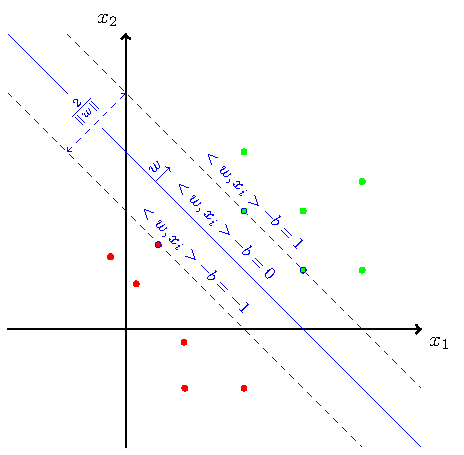
\includegraphics[width=0.5\textwidth]{Figure_SVM}
	\caption{Nun wurden zu der Trenngerade zwischen den Datensätzen noch zwei parallele Geraden hinzugefügt, die als Stützvektoren (Support vectors) einen der klassifizierten Datenpunkte nutzen. Dann lässt sich das mathematische Programm optimieren.}
	\label{SVM2}
	\end{center}
\end{dsafigure}

\section{Neuronale Netze}

%Das ist ein Kommentar 

\subsection{Einführung}

Inspiriert von unserem Verständnis, wie das menschliche Gehirn lernt, benutzen Neuronale Netze Lernalgorithmen, welche besonders für praktische Anwendungen geeignet sind.
Dazu zählen Spracherkennung, Objekterkennung in Bildern und die Fähigkeit individüll passende Produkte vorzuschlagen, die dem Kunden gefallen könnten. 
Ein Neuronales Netz wird von mehreren Schichten aufgebaut. Ausgangsschicht ist dabei, die Datenschicht, auf die ein oder mehrere hidden layer folgen. Als Ausgabewert erhält man schließlich einen Vektor, welcher die Wahrscheinlichkeitsverteilung darstellt. Mit anderen Worten, wie wahrscheinlich es ist, dass das Ausgangsobjekt zu einer bestimmten Klasse gehört.

\begin{dsafigure}
\begin{center}
	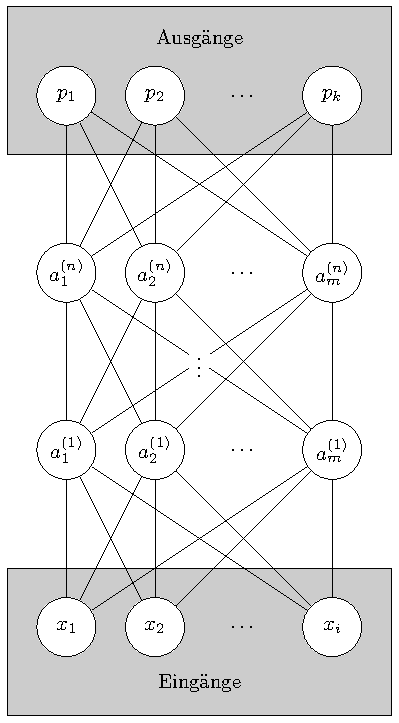
\includegraphics[width=0.5\textwidth]{Figure_NN}
	\caption{ASHGDXJAGSHDJAGSDJAGS}
	\label{NN1}
	\end{center}
\end{dsafigure}

\subsection{SVMs als Neuronale Netze}

Wir haben bereits SVMs kennengelernt. Im folgenden wird verdeutlicht, wie man diese auch als Neuronales Netz ausdrücken kann. Charakteristisch für dieses Neuronale Netz ist, dass es nur einen Layer besitzt:

\begin{equation*}
\min\limits_{b,w,z} \norm{w} + C * \sum * z
\end {equation*}

sodass:

\begin{equation*}
y_i (<w,x> - b) \geq 1 - z ; z_i \geq 0 => z_i \geq 1- y_i (<w,x> - b); z_i \geq 0
\end {equation*}

\begin{equation*}
\min \norm{w} + C \cdot \sum \max (0, 1-y_i (<w,x_i>-b) = \norm{w} + C \sum \ell ( 1-y_i (<w,x_i>)-b) = \norm{w} + C \sum \ell (a_i)
\end{equation*}

\subsection{Lineare Regression}

Auch die lineare Regression kann auch in Form von Neuronalen Netzen ausgedrückt werden. Der wesentliche Unterschied dabei ist, dass keine Klassifikation stattfindet, sondern den Datensätzen konkrete Werte zugeordnet werden.

\begin{equation*}
\min\limits{w,b} 0,5 \sum ((<w,x_i> - b) -y_i)^2
a_i = <w,x_i> -b-y_i
\end{equation*}

\subsection{Deep Learning}

Mit Deep Learing beschreibt man die Neuronalen Netze, die über mehr als einen hidden layer verfügen. Dabei wird jeweils eine nicht lineare Funktion auf die linearen Ergebnisse der einzelnen layer angewendet, um die Anzahl der Parameter zu vergrößern.

\subsection{Convolutional Neuronal Networks}
